\documentclass{article}
\usepackage{changepage}
\usepackage{graphicx}
\usepackage{hyperref}

\textwidth=6.25in
\textheight=9.5in
\headheight=0in
\headsep=.5in
\hoffset  -1in
\topmargin -.75in

\nofiles

%\setlength{\parskip}{0.0cm}
%\setlength{\parindent}{0.0cm}   % Don't indent the paragraphs

% \begin{adjustwidth}{2em}{0pt}
% \end{adjustwidth}

\begin{document}
\begin{flushright}
    Matt Gautreau\\
    Zach Montoya\\
    CS 422\\
    Final Project Report
\end{flushright}

\section{Overview}

MYRC is a Java-based distributed chat application which seeks to implement
a subset of the IRC protocol as faithfully as possible. The implementation
includes both server and client programs, and facilitates client-server, and
client-client(s) communication through the server. This communication is
done using sockets.

\section{System Architecture}

The general structure of the system is as follows:

\begin{center}
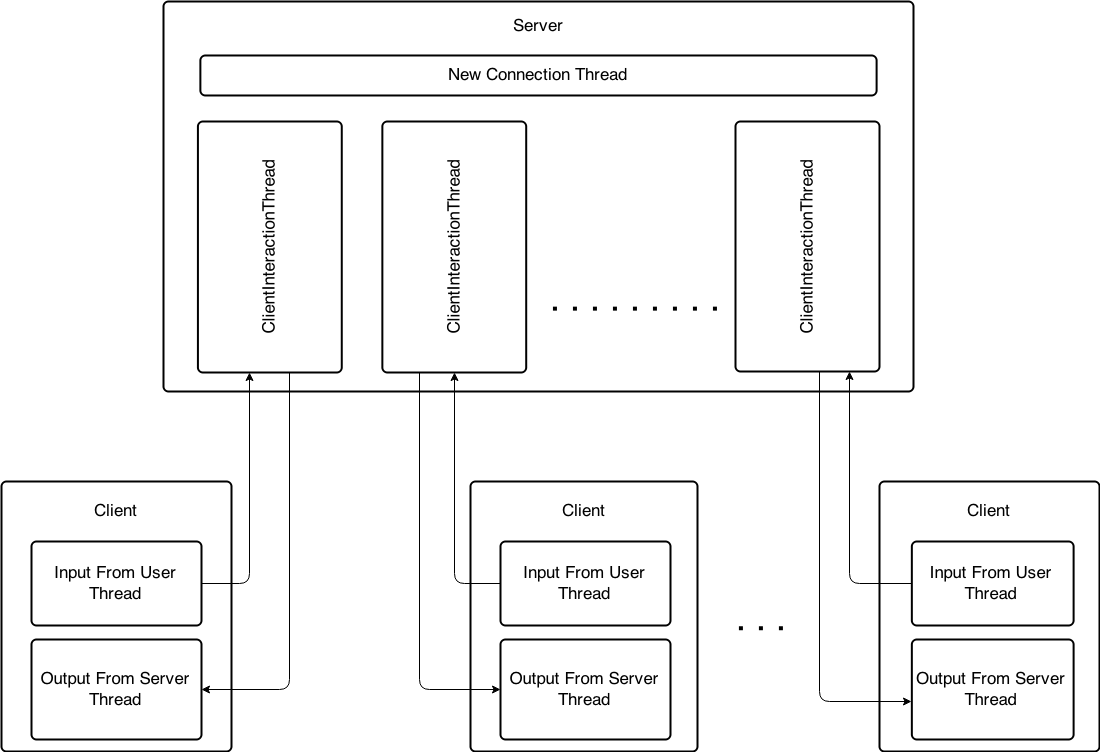
\includegraphics[width=\linewidth]{architecture.png}
\end{center}

\subsection{Server Architecture}

The IRC protocol specifies that servers manage a set of chatrooms, called channels,
which have the following fundamental properties:
\begin{enumerate}
    \item
        Name - usually indicative of the topic of the channel
    \item
        Topic - a brief explanation of the channel's purpose
    \item
        Users - a set of users currently in the channel
\end{enumerate}

Users must be able to send messages both to other users and to an entire channel.
For this purpose, the server maintains a collection of all channels it is currently
managing, as well as the collection of all users that are connected to the server.

The main server thread, labeled ``New Connection Thread'' in the architecture diagram,
simply exists to constantly wait for a connection to the \texttt{ServerSocket}.  When
a new client connects, we create a socket assigned to that particular client, a \texttt{UserInfo}
object associated with the connecting user, and then start a \texttt{ClientInteractionThread}
to handle server-client communication with the new client.
\\

The \texttt{ClientInteractionThread} will constantly wait to receive a message from
the client, parse that message, and perform the action associated with the message.
Any responses that are generated while executing the message will be sent back to
the client.

\subsection{Client Architecture}

On startup, the client will connect to the server via the server's new connection thread.
Once a connection is established, the client will
create two threads.  One thread will be waiting for user input (in the form of an IRC message)
and sending it over its socket to its corresponding \texttt{ClientInteractionThread} on the server.
The other thread will be responsible for receiving chats or other responses from the server, and printing
them so the user may see them on \texttt{stdout}.

\subsection{Message Handling}

MYRC currently supports the following IRC commands. Since our implementation is
limited, each command will contain a description of the precise way in which it
is handled in our system.
\begin{itemize}
    \item PASS: The first of two commands to register a user.
    \item USER: The second of two commands to register a user. Sets the realname for
    the client and the unique nickname for the client.
    \item NICK: Sets the unique nickname for the client.
    \item JOIN: If the target channel exists, the user joins the specified channel
    and receives all updates from the channel.
    \item PRIVMSG: Allows the user to send a message to another user or channel,
    if the target exists.
    \item TOPIC: Allows the user to set or get the topic of a channel if they
    have already joined.
    \item PART: Allows the user to leave a channel that they had already joined.
\end{itemize}

The message handling system is as follows.  The raw string of a message has an associated
grammar.  We use this grammar to parse the message, which then contains a \texttt{command}
field, in addition to components called \texttt{parameters}, \texttt{prefix}, and \texttt{trailing}.
The \texttt{command} field is used to determine which of the above message types it is.
We have an abstract class called \texttt{Message}, which contains all the fields of the message,
and includes an abstract method called \texttt{executeCommand}.  We then create extensions of the
abstract class for each of the supported commands, implementing the \texttt{executeCommand} in
accordance with the behavior of the message as defined in the IRC protocol.




\end{document}
